\chapter{Bose统计和Fermi统计}

即使粒子间相互作用可以忽略，理想气体在低温或高密度下也可能不满足非简并条件。此时必须保留量子统计效应，分别采用Bose分布和Fermi分布：
\begin{equation}
	a_i=\frac{\omega_i}{\e^{\alpha+\beta\varepsilon_i}\pm 1},
\end{equation}
约定
$\pm$号的($+$)对应Fermi分布，($-$)对应Bose分布。
$\mp$号反之。

\begin{definition}{巨配分函数}{grand partition function}
	定义巨配分函数(grand partition function)的对数
	\begin{equation}
		\ln\Xi:=\pm\sum_i\omega_i\ln(1\pm\e^{-\alpha-\beta\varepsilon_i}),
	\end{equation}
\end{definition}

\begin{corollary}
	以$\alpha,\beta$和外参量$\{y_k\}$为独立变量。用$N$表示平均粒子数，$a_i$表示能级$i$的平均占据数。根据巨配分函数可导出粒子数、内能、状态方程和熵等宏观量：
	\begin{subequations}
		\begin{align}
			N&=-\pv{\ln\Xi}\alpha,\\
			U&=-\pvat{\ln\Xi}{\beta}{\alpha,\{y_k\}},\\
			Y_k&=-\frac1\beta\pv{\ln\Xi}{y_k},\\
			S&=\kB(\ln\Xi+\alpha N+\beta U),\\
			\mu&=-\alpha\kB T.
		\end{align}
	\end{subequations}
\end{corollary}

\begin{proof}
	粒子数
	\[
		N=\sum_i a_i=\sum_i\frac{\omega_i}{\e^{\alpha+\beta\varepsilon_i}\pm 1}=\mp\sum_i\omega_i\pp\alpha{\ln(1\pm\e^{-\alpha-\beta\varepsilon_i})}=-\pv{\ln\Xi}\alpha,
	\]
	内能
	\[
		U=\sum_i a_i\varepsilon_i=\sum_i\frac{\omega_i\varepsilon_i}{\e^{\alpha+\beta\varepsilon_i}\pm 1}=\mp\sum_i\omega_i\pp\beta{\ln(1\pm\e^{-\alpha-\beta\varepsilon_i})}=-\pv{\ln\Xi}\beta,
	\]
	状态方程
	\[
		Y_k=\sum_i a_i\pv{\varepsilon_i}{y_k}=\mp\frac1\beta\sum_i\omega_i\pp{y_k}{\ln(1\pm\e^{-\alpha-\beta\varepsilon_i})}=-\frac1\beta\pv{\ln\Xi}{y_k},
	\]
	微观态$s$的归一化概率为$P_s=\Xi^{-1}\e^{-\alpha N_s-\beta E_s}$。其统计熵为
	\[
		S=-\kB\sum_s P_s\ln P_s=\kB(\ln\Xi+\alpha N+\beta U).
	\]
	由以上三个偏导数，
	\begin{align*}
		\d\ln\Xi&=-N\d\alpha-U\d\beta-\beta\sum_k Y_k\d y_k,\\
		\d S&=\kB\left[\beta\left(\d U-\sum_kY_k\d y_k\right)+\alpha\d N\right].
	\end{align*}
	与热力学基本方程比较，得到$\beta=1/(\kB T)$、$\alpha=-\beta\mu$。若改用$\mu,\beta$为独立变量，则固定$\mu$时有$-(\partial\ln\Xi/\partial\beta)_{\mu,\{y_k\}}=U-\mu N$。
\end{proof}

\begin{corollary}
	当能谱可作连续近似时，$\ln\Xi$、粒子数$N$和内能$U$可以写成态密度$g(\varepsilon)$的积分。具有宏观占据数的离散能级须单独求和。
	\begin{subequations}
		\begin{align}
			\ln\Xi&=\pm\intRplus g(\varepsilon)\ln(1\pm\e^{-\alpha-\beta\varepsilon})\d\varepsilon,\\
			N&=-\pv{\ln\Xi}\alpha=\intRplus\frac{g(\varepsilon)}{\e^{\alpha+\beta\varepsilon}\pm 1}\d\varepsilon,\\
			U&=-\pv{\ln\Xi}\beta=\intRplus\frac{g(\varepsilon)\varepsilon}{\e^{\alpha+\beta\varepsilon}\pm 1}\d\varepsilon.
		\end{align}
	\end{subequations}
\end{corollary}

\section{弱简并理想Bose气体和Fermi气体}
\label{sec:weak degeneracy}

\paragraph{弱简并条件}

取基态能量为零。弱简并气体中，量子交换给经典热力学量带来小修正，可以对逸度$\e^{-\alpha}$展开。以下幂级数在$\e^{-\alpha}<1$时收敛。只保留前一两项还要求逸度足够小。
\exmref{exm:monatomic molecule} 已给出单原子气体平动的态密度：
\[
	g(\varepsilon)=g_s\frac{2\pi V}{h^3}(2m)^{3/2}\sqrt\varepsilon,
\]
上式考虑了自旋因子$g_s$，因此巨配分函数的对数为
\[
	\ln\Xi=\pm 2\pi g_sV\biggp{\frac{2m}{h^2}}^{3/2}\intRplus\sqrt\varepsilon\ln(1\pm\e^{-\alpha-\beta\varepsilon})\d\varepsilon.
\]
由于$\e^{-\alpha-\beta\varepsilon}\leq\e^{-\alpha}<1$，积分中的$\ln$项可写成级数形式：
\[
	\ln(1\pm x)=-\sum_{k=1}^\infty\frac{(\mp x)^k}k.
\]
交换积分和级数求和，可得
\begin{align*}
	\ln\Xi
	&=\mp 2\pi g_sV\biggp{\frac{2m}{h^2}}^{3/2}\sum_{k=1}^\infty\frac{(\mp\e^{-\alpha})^k}{k}\intRplus\sqrt\varepsilon\e^{-k\beta\varepsilon}\d\varepsilon\\
	&=\mp 2\pi g_sV\biggp{\frac{2m}{h^2}}^{3/2}\sum_{k=1}^\infty\frac{(\mp\e^{-\alpha})^k}{k}\frac{\sqrt\pi}{2(k\beta)^{3/2}}
	=\mp g_sV\biggp{\frac{2\pi m}{h^2\beta}}^{3/2}\Li_{5/2}(\mp\e^{-\alpha}).
\end{align*}
这里引入了多重对数函数(polylogarithm)
\begin{equation}
	\Li_n(z):=\sum_{k=1}^\infty\frac{z^k}{k^n}.
\end{equation}
% 特别地$\Li_{5/2}(1)=\zeta(5/2)\approx 1.3415,\,\Li_{5/2}(-1)=-(1-2^{-3/2})\zeta(5/2)\approx-0.8672$。
由$\d\Li_n(\e^{-x})/\nd x=-\Li_{n-1}(\e^{-x})$，可得粒子数
\[
	N=-\pv{\ln\Xi}\alpha=\mp g_sV\biggp{\frac{2\pi m}{h^2\beta}}^{3/2}\Li_{3/2}(\mp\e^{-\alpha}).
	% \xi=\frac{nh^3}{g_s(2\pi m\kB T)^{3/2}}.
\]
即
\[
	\ln\Xi=N\frac{\Li_{5/2}(\mp\e^{-\alpha})}{\Li_{3/2}(\mp\e^{-\alpha})}.
\]
% 由
% \[
% 	\frac{\Li_n(x)}{\Li_{n-1}(x)}=1-2^{-n}x-2(3^{-n}-4^{-n})x^2+\bigo(x^3),
% \]
内能、压强和熵等宏观量为
\begin{subequations}
	\begin{align}
		U&=-\pv{\ln\Xi}\beta=\frac32\frac{\ln\Xi}\beta=\frac32N\kB T\frac{\Li_{5/2}(\mp\e^{-\alpha})}{\Li_{3/2}(\mp\e^{-\alpha})},\\
		C_V&=\pvat{U}{T}{V}=\frac32N\kB\biggb{\frac{5}2\frac{\Li_{5/2}(\mp\e^{-\alpha})}{\Li_{3/2}(\mp\e^{-\alpha})}-\frac32\frac{\Li_{3/2}(\mp\e^{-\alpha})}{\Li_{1/2}(\mp\e^{-\alpha})}},\\
		p&=\frac1\beta\pv{\ln\Xi}V=\frac23\frac UV=\frac{N\kB T}V\frac{\Li_{5/2}(\mp\e^{-\alpha})}{\Li_{3/2}(\mp\e^{-\alpha})},\\
		S&=\kB(\ln\Xi+\alpha N+\beta U)=\alpha N\kB+\frac53\frac UT=N\kB\biggb{\alpha+\frac52\frac{\Li_{5/2}(\mp\e^{-\alpha})}{\Li_{3/2}(\mp\e^{-\alpha})}}.
	\end{align}
\end{subequations}
其中$C_V$在固定$N,V$下计算，$\alpha$随$T$调整以保持数密度$n$不变。于是
\[
	C_V=\frac32N\kB\pp T\biggp{T\frac{\Li_{5/2}(\mp\e^{-\alpha})}{\Li_{3/2}(\mp\e^{-\alpha})}}=\frac32N\kB\biggb{\frac{\Li_{5/2}(\mp\e^{-\alpha})}{\Li_{3/2}(\mp\e^{-\alpha})}+T\pp T\frac{\Li_{5/2}(\mp\e^{-\alpha})}{\Li_{3/2}(\mp\e^{-\alpha})}}.
\]
而
\[
	T=\frac{h^2}{2\pi m\kB}\biggp{\frac{n}{\mp g_s\Li_{3/2}(\mp\e^{-\alpha})}}^{2/3}
	\implies
	T\pp T=T\pv\alpha T\pp\alpha=\frac32\frac{\Li_{3/2}(\mp\e^{-\alpha})}{\Li_{1/2}(\mp\e^{-\alpha})}\pp\alpha.
\]
注意系数$3/2$来自指数$-2/3$而不是$\Li_{3/2}$的底数。
再直接对$\alpha$求导即得$C_V$表达式。

\paragraph{对$\e^{-\alpha}$或$\xi$展开}

定义$\xi:=n\lambda_T^3/g_s=\mp\Li_{3/2}(\mp\e^{-\alpha})$，
利用
\[
	\Li_n^{-1}(x)=x-2^{-n}x^2+(2^{1-2n}-3^{-n})x^3+\bigo(x^4),
\]
可得$\e^{-\alpha}=\mp\Li_{3/2}^{-1}(\mp\xi)$，
进而$\ln\Xi=\mp N\Li_{5/2}(\Li_{3/2}^{-1}(\mp\xi))/\xi$，
由
\[
	\Li_n(\Li_{n-1}^{-1}(x))=x-2^{-n}x^2-(2\cdot 3^{-n}-4^{1-n})x^3+\bigo(x^4),
\]
将$\ln\Xi$和宏观量写成$\e^{-\alpha}$或$\xi$的级数形式：
\begin{subequations}
	\begin{align}
		U&=\frac32N\kB T(1\pm 2^{-5/2}\e^{-\alpha}+\cdots)=\frac32N\kB T(1\pm 2^{-5/2}\xi+\cdots),\\
		C_V&=\frac32N\kB(1\mp 2^{-7/2}\e^{-\alpha}+\cdots)=\frac32N\kB(1\mp 2^{-7/2}\xi+\cdots),\\
		p&=\frac{N\kB T}V(1\pm 2^{-5/2}\e^{-\alpha}+\cdots)=\frac{N\kB T}V(1\pm 2^{-5/2}\xi+\cdots),\\
		S&=N\kB\biggp{\alpha+\frac52\pm 5\cdot2^{-7/2}\e^{-\alpha}+\cdots}=N\kB\biggp{\frac52-\ln\xi\pm 2^{-7/2}\xi+\cdots}.
	\end{align}
\end{subequations}

\begin{corollary}
	比较$N,V,T$、粒子质量和内态简并度相同的气体，首阶交换修正给出$U,p,S$的次序为Fermi $>$半经典$>$ Bose，$C_V$的次序相反。
\end{corollary}

\begin{remark}
	强简并条件下，Bose气体和Fermi气体性质完全不同。
	这是因为：Bose子有可能大量占据低能态，形成Bose--Einstein凝聚；而Fermi子由于Pauli原理，低能态被填满后只能占据高能态，导致零点能和简并压等现象。
	取基态能量为零，有限系统中Bose气体的$\alpha>0$，而Fermi气体的$\alpha$可正可负。对于Fermi气体，$\alpha<0$时多重对数的自变量$-\e^{-\alpha}<-1$，可用解析延拓或直接用能量积分计算宏观量。
\end{remark}

\section{量子交换关联与粒子符合计数}
\label{sec:exchange-correlations}

在给定空间分辨率下，单粒子探测的平均计数正比于探测体积内的平均粒子数。在$\bm r_1$记录到一个粒子后，$\bm r_2$附近记录到另一个粒子的概率会怎样改变？记同一时刻在$\bm r_j$湮灭一个粒子的场算符为$\hat\psi_j$，相应的产生算符为$\hat\psi_j^\dagger$，局域数密度为$n_j=\ave{\hat\psi_j^\dagger\hat\psi_j}$。用独立探测的概率归一化双粒子符合计数，得到无量纲的二阶关联函数
\begin{equation}
	g^{(2)}(\bm r_1,\bm r_2)=
	\frac{\ave{\hat\psi_1^\dagger\hat\psi_2^\dagger\hat\psi_2\hat\psi_1}}{n_1n_2}.
\end{equation}
分子中的两个湮灭算符依次移去两个粒子。这一排列剔除了同一粒子与自身配对的计数。彼此独立的两次探测给出$g^{(2)}=1$。

考虑处于巨正则热平衡的单组分理想气体，设哈密顿量与总粒子数算符对易，Bose气体处于未凝聚的正常相。理想气体的哈密顿量是场算符的二次型，其热态为高斯态，四个场算符的平均可用Wick定理分解。由于热态在整体相位变换下不变，改变总粒子数的配对平均$\ave{\hat\psi_1\hat\psi_2}$为零。记一阶关联$G^{(1)}_{12}=\ave{\hat\psi_1^\dagger\hat\psi_2}$。直接配对给出$n_1n_2$，交换配对给出$G^{(1)}_{12}G^{(1)}_{21}$，交换两个Fermi算符还会产生一个负号。因此
\begin{equation}
	\label{eqn:exchange coincidences}
	g^{(2)}(\bm r_1,\bm r_2)=1+\eta\,\frac{\abs{G^{(1)}_{12}}^2}{n_1n_2},
	\qquad \eta=\begin{cases}
		+1,&\text{Bose子},\\
		-1,&\text{Fermi子}.
	\end{cases}
\end{equation}
当两点重合时，$G^{(1)}_{11}=n_1$。单组分混沌热Bose气体的$g^{(2)}(0)=2$，即\textbf{聚束}。自旋极化理想Fermi气体的$g^{(2)}(0)=0$，即\textbf{反聚束}。若探测器同时接收多个内态，不同内态之间的符合计数会减弱这一交换信号。Bose子的聚束还取决于制备的态。例如$N$个粒子全部占据同一轨道时，可计数的有序粒子对有$N(N-1)$个，因而$g^{(2)}=1-1/N$。

在均匀非简并气体中，各动量的权重由Maxwell分布给出。设$\bm r=\bm r_2-\bm r_1$，对动量分布作归一化的Fourier变换，可得交换关联的空间范围
\[
	\frac{G^{(1)}_{12}}{n}\simeq
	\frac{\int \d^3p\,\e^{-\beta p^2/(2m)}\e^{\i\bm p\cdot\bm r/\hbar}}
	{\int \d^3p\,\e^{-\beta p^2/(2m)}}=\e^{-\pi r^2/\lambda_T^2}.
\]
故$g^{(2)}(r)-1\simeq\eta\exp(-2\pi r^2/\lambda_T^2)$。即使交换效应对压强的修正已经很小，间距小于热波长的粒子对仍然表现出可测的关联。

在原子的Hanbury Brown--Twiss实验中，Jeltes等用同一套装置分别释放自旋极化的亚稳态$^4\mathrm{He}$和$^3\mathrm{He}$原子云，逐个记录原子的到达位置和时刻。小间距处，未凝聚的$^4\mathrm{He}$在符合计数中形成峰，$^3\mathrm{He}$形成谷。探测器的有限分辨率使测得的关联在一段间距上取平均，因而降低了峰、谷相对于$1$的对比度。\footnote{\href{https://doi.org/10.1038/nature05513}{T.~Jeltes等，Nature \textbf{445}, 402--405 (2007)}，见图2。}

\section{Bose气体}

\subsection{Bose--Einstein凝聚}

考虑三维均匀理想Bose气体，取基态能量$\varepsilon_0=0$，基态简并度为$\omega_0$。在有限体积、$T>0$时，每个单粒子态的巨配分函数都是收敛的几何级数，要求$\mu<\varepsilon_0$。令逸度$q=\e^{\beta\mu}=\e^{-\alpha}<1$，把固定的平均粒子数分为基态和激发态两部分：
\[
	N=N_0+N_+,\qquad N_0=\frac{\omega_0 q}{1-q},\qquad
	N_+=\sum_{i>0}\frac{\omega_i}{q^{-1}\e^{\beta\varepsilon_i}-1}.
\]
在热力学极限$N,V\to\infty$、$n=N/V$固定时，对激发态作连续近似。给定温度下，激发态密度随$q$增大而增大，并在$q\to1^-$时达到上限：
\[
	\frac{N_+}{V}=\frac{g_s}{\lambda_T^3}\Li_{3/2}(q)
	\ \longrightarrow\ \frac{g_s}{\lambda_T^3}\zeta\biggp{\frac32}.
\]
由于$\lambda_T^{-3}\propto T^{3/2}$，降温时这个上限不断降低。当它等于总密度$n$时，温度达到临界值
\begin{equation}
	\label{eqn:Bose TC}
	T_\criticalpoint=\frac{h^2}{2\pi m\kB}\biggp{\frac n{\zeta(3/2)g_s}}^{2/3}.
\end{equation}

\paragraph{低温下的Bose--Einstein凝聚}

$T<T_\criticalpoint$时，激发态达到饱和，其余粒子宏观占据基态，这称为\textbf{Bose--Einstein凝聚} (Bose--Einstein condensation, BEC)。在热力学极限中，由饱和密度可得
\begin{equation}
	\frac{N_+}N=\biggp{\frac T{T_\criticalpoint}}^{3/2},\qquad
	\frac{N_0}N=1-\biggp{\frac{T}{T_\criticalpoint}}^{3/2}.
\end{equation}
在这一温区取定$T$并增大体积，$N_0$正比于$V$。由有限体系的基态占据数可反解得
\[
	\mu=-\kB T\ln\biggp{1+\frac{\omega_0}{N_0}}\to0^-,\qquad
	\ln\Xi_0=-\omega_0\ln(1-q)=\omega_0\ln\biggp{1+\frac{N_0}{\omega_0}}.
\]
基态在粒子数中占有限比例，而$\ln\Xi_0/V\to0$。因此$\ln\Xi$正比于体积的主项来自激发态：
\begin{equation}
	\ln\Xi\simeq-\intRplus g(\varepsilon)\ln(1-\e^{-\beta\varepsilon})\d\varepsilon
	=\zeta\biggp{\frac52}\frac{g_sV}{\lambda_T^3}.
\end{equation}
在这个极限下，可得$T<T_\criticalpoint$时的内能、热容、压强和熵等物理量：
\begin{subequations}
	\begin{align}
		U&=-\pv{\ln\Xi}\beta=\frac32\frac{\ln\Xi}\beta=\frac{3\zeta(5/2)}{2\zeta(3/2)}N\kB T\biggp{\frac T{T_\criticalpoint}}^{3/2},\\
		C_V&=\pvat{U}{T}{V}=\frac52\frac UT=\frac{15\zeta(5/2)}{4\zeta(3/2)}N\kB\biggp{\frac T{T_\criticalpoint}}^{3/2},\\
		p&=\frac1\beta\pv{\ln\Xi}V=\frac23\frac UV=\frac{\zeta(5/2)}{\zeta(3/2)}\frac{N\kB T}V\biggp{\frac T{T_\criticalpoint}}^{3/2},\\
		S&=\kB(\ln\Xi+0+\beta U)=\frac53\frac UT=\frac{5\zeta(5/2)}{2\zeta(3/2)}N\kB\biggp{\frac T{T_\criticalpoint}}^{3/2},\\
		F&=U-TS=-\frac23U,\\
		G&=F+pV=0\implies\mu=0.
	\end{align}
\end{subequations}

\paragraph{相变点的比热}
$T<T_\criticalpoint$时，比热$C_V\propto T^{3/2}$；
$T>T_\criticalpoint$时，由\secref{sec:weak degeneracy}的多重对数表达式，
\[
	C_V=\frac32N\kB\biggb{\frac52\frac{\Li_{5/2}(\e^{-\alpha})}{\Li_{3/2}(\e^{-\alpha})}-\frac32\frac{\Li_{3/2}(\e^{-\alpha})}{\Li_{1/2}(\e^{-\alpha})}},
\]
$T\to T_\criticalpoint^+$时，$\alpha=-\beta\mu\to0^+$，$q=\e^{-\alpha}\to1^-$。$\Li_{5/2}(q)$和$\Li_{3/2}(q)$分别趋于$\zeta(5/2)$和$\zeta(3/2)$，而$\Li_{1/2}(q)=\sum_{k=1}^\infty q^k/\sqrt{k}$趋于无穷，故
\[
	\lim_{T\to T_\criticalpoint^+}\frac{C_V}{N\kB}
	=\frac{15}4\frac{\zeta(5/2)}{\zeta(3/2)}
	=\lim_{T\to T_\criticalpoint^-}\frac{C_V}{N\kB}\approx1.926.
\]
热容在临界点连续，两侧曲线在这里形成尖峰。高温极限下，$\e^{-\alpha}\to0$，
\[
	\lim_{T\to+\infty}C_V=\biggp{\frac{15}4-\frac94}N\kB=\frac32N\kB.
\]


\begin{notecaptionblock}
	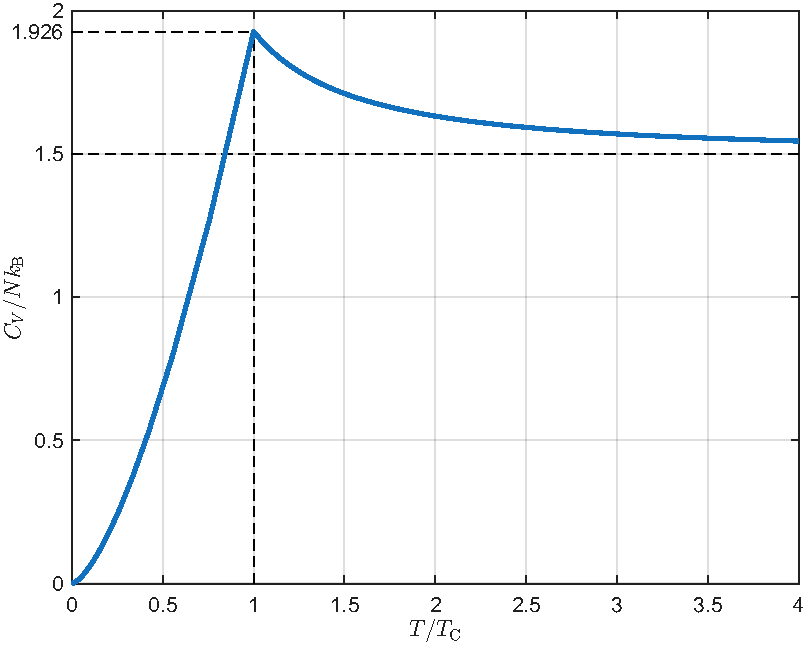
\includegraphics[width=0.7\linewidth]{figures/C_VBoson.pdf}
	\captionof{figure}{理想Bose气体热容$C_V$随温度的变化}
\end{notecaptionblock}

\begin{remark}
	% 由于历史条件，当时还不知道全同多粒子系存在（量子起源的）统计关联：对Bose子是有效吸引；而Fermi子是有效排斥。因此，即使没有动力学相互作用，仍可在一定条件下由于有效相互作用而发生凝聚现象。这是一种纯粹量子起源的相变。
	
	实现Bose--Einstein凝聚极其困难，原则上要使气体冷却至
	$n\lambda_T^3/g_s\geq\zeta(3/2)\approx 2.612$，
	但大多数情况下，在远高于BEC的$T_\criticalpoint$到达以前，已发生液化甚至固化的相变。为了实现原子气体的BEC，必须用极稀薄的气体，且要求
	\begin{center}
		二体弹性碰撞的弛豫时间$\ll$形成分子集团的非弹性碰撞的弛豫时间
	\end{center}
	对于碱金属原子气体，前者$\sim\qty{10}{\milli\second}$，而后者有几秒至几分钟。%$\tau_\mathrm{elas}\ll$$\tau_\mathrm{inelas}$
	
	% BEC-BCS Crossover Fermionic condensation.
\end{remark}

\subsection{弱相互作用Bose气体与超流}
\label{sec:bogoliubov-gas}

均匀气体发生凝聚后，若使其相对容器运动，它能否产生激发而损失动能？要回答这个问题，需要求流体静止时的激发能$E(p)$。取三维、接近零温的单组分Bose气体，设原子质量为$m$，排斥作用的$s$波散射长度为$a_s>0$。在$n a_s^3\ll1$且波长远大于势的作用范围时，低能两体碰撞可用接触耦合常数$g=4\pi\hbar^2a_s/m$描述。设凝聚体密度为$n_0$，在弱耗尽近似中$n_0\simeq n$。

凝聚波函数$\Phi(\bm r,t)$满足Gross--Pitaevskii方程
\[
	\i\hbar\pv{\Phi}{t}=\left(-\frac{\hbar^2}{2m}\nabla^2+g\abs{\Phi}^2\right)\Phi .
\]
均匀解为$\Phi_0=\sqrt{n_0}\e^{-\i\mu t/\hbar}$，其中$\mu=gn_0$。写成$\Phi=\e^{-\i\mu t/\hbar}(\sqrt{n_0}+\delta\phi)$，只保留扰动的一次项，得
\[
	\i\hbar\pv{\delta\phi}{t}
	=\left(-\frac{\hbar^2}{2m}\nabla^2+gn_0\right)\delta\phi+gn_0\,\delta\phi^* .
\]
密度扰动引起的平均势变化把$\delta\phi$与其复共轭耦合起来。令$\theta=\bm p\cdot\bm r/\hbar-\omega t$，代入$\delta\phi=u\e^{\i\theta}+v^*\e^{-\i\theta}$，并记$\varepsilon_p=p^2/(2m)$，两项的系数满足
\[
	\begin{pmatrix}
		\varepsilon_p+gn_0 & gn_0\\
		-gn_0 & -\varepsilon_p-gn_0
	\end{pmatrix}
	\begin{pmatrix}u\\v\end{pmatrix}
	=\hbar\omega\begin{pmatrix}u\\v\end{pmatrix}.
\]
特征方程给出$(\hbar\omega)^2=(\varepsilon_p+gn_0)^2-(gn_0)^2$。一个正频率模式的激发能构成\textbf{Bogoliubov谱}
\begin{equation}
	\label{eqn:bogoliubov spectrum}
	E(p)=\sqrt{\varepsilon_p(\varepsilon_p+2gn_0)}
	=p\sqrt{c^2+\left(\frac{p}{2m}\right)^2},\qquad c=\sqrt{\frac{gn_0}{m}}.
\end{equation}
长波端$\varepsilon_p\ll gn_0$时，密度扰动以声速$c$传播，$E(p)\simeq cp$。当$\varepsilon_p\gg gn_0$且接触相互作用近似仍成立时，$E(p)=\varepsilon_p+gn_0+\bigo((gn_0)^2/\varepsilon_p)$，能量的主项恢复为单粒子的动能。\footnote{凝聚体的小涨落展开见T.~Senthil的\href{https://ocw.mit.edu/courses/8-513-many-body-theory-for-condensed-matter-systems-fall-2004/resources/notes6/}{MIT 8.513多体理论讲义，第6讲}。}
\begin{notecaptionblock}
	\tikzfigure{bogoliubov-spectrum}
	\captionof{figure}[弱排斥Bose气体的Bogoliubov谱]{弱排斥Bose气体的Bogoliubov谱与长波声学色散$cp$、自由粒子动能$p^2/(2m)$。两条参考曲线分别给出低动量和高动量时的主项。}
	\label{fig:bogoliubov-spectrum}
\end{notecaptionblock}

在流体静止系中，设一个重障碍物以速度$\bm v$运动。若它向流体传递动量$\bm p$，忽略障碍物的反冲修正，其提供的能量为$\bm v\cdot\bm p$。能量守恒要求$\bm v\cdot\bm p\ge E(p)$，所以零温下通过这一激发分支耗散的速度阈值满足\textbf{Landau判据}
\[
	v_{\mathrm L}=\inf_{p>0}\frac{E(p)}{p}.
\]
对式\eqref{eqn:bogoliubov spectrum}取下确界可得$v_{\mathrm L}=c$，首先允许产生的是长波声子。令$g=0$，理想气体在零温仍有宏观凝聚占据，但其抛物线色散给出$v_{\mathrm L}=0$。凝聚分数由单粒子态的占据决定，产生激发的速度阈值由能量与动量之比决定。实际容器中，边壁附近的涡旋成核还可能使观测到的耗散阈值低于$c$。

\subsection{光子气体}

黑体空腔的腔壁可吸收和发射光子，给定$T,V$后，光子总数由热平衡决定，因而没有固定粒子数迫使激发态饱和的约束。光子的能量与动量满足相对论关系
\begin{align}
	\varepsilon=h\nu=cp.
\end{align}
忽略光子间的相互作用，取黑体辐射平衡时的$\mu=0$、$\alpha=0$，得到
\[
	a_i=\frac{\omega_i}{\e^{\beta\varepsilon_i}-1}.
\]
\begin{theorem}
	{Planck黑体辐射定律}{Planck blackbody radiation}
	能完全吸收电磁波的物体，称为黑体。黑体辐射的能量谱为
	\begin{subequations}
		\begin{align}
			u(\nu)\d\nu&=\frac{8\pi h\nu^3}{c^3}\frac1{\e^{\beta h\nu}-1}\d\nu,\\
			u(\lambda)\d\lambda&=\frac{8\pi hc}{\lambda^5}\frac1{\e^{\beta hc/\lambda}-1}\d\lambda.
		\end{align}
	\end{subequations}
	\begin{notecaptionblock}
		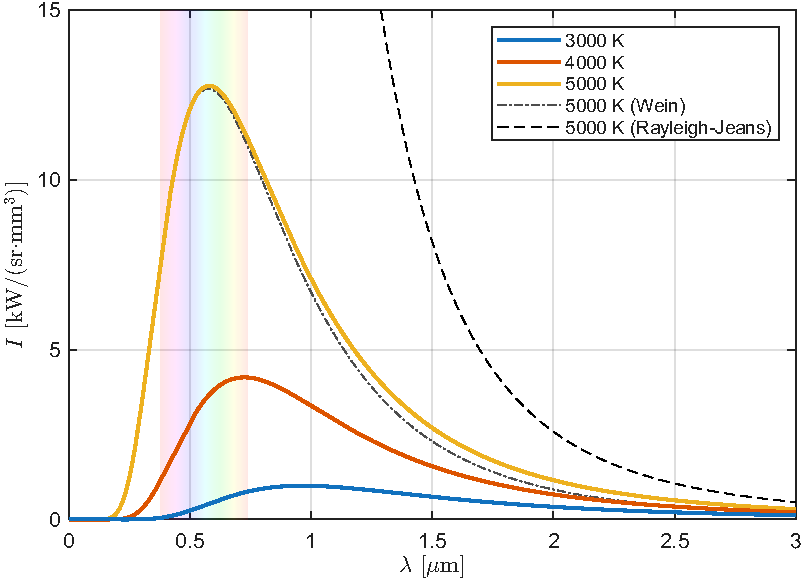
\includegraphics[width=0.8\linewidth]{figures/blackbody.pdf}
	\captionof{figure}[不同温度下黑体的谱辐亮度]{不同温度下黑体的谱辐亮度 $B_\lambda$。各向同性的黑体辐射场满足 $u(\lambda)=4\pi B_\lambda/c$。}
		\label{fig:blackbody radiation}
	\end{notecaptionblock}
\end{theorem}

\begin{proof}
	假设$V$很大，能量准连续，$(\nu,\nu+\d\nu)$内的微观状态数
	\[
		g(\varepsilon)\d\varepsilon=\frac{g_sV}{h^3}\frac{4\pi}{c^3}\varepsilon^2\d\varepsilon\implies g(\nu)\d\nu=g(h\nu)h\d\nu=\frac{4\pi g_sV}{c^3}\nu^2\d\nu.
	\]
	其中光子的自旋因子$g_s=2$，
	光子数
	\[
		N(\nu)\d\nu=\frac{g(\nu)\d\nu}{\e^{\beta h\nu}-1}.
	\]
	可得能量谱
	\[
		u(\nu)\d\nu=\frac{N(\nu)}Vh\nu\d\nu=\frac{h\nu}V\frac{g(\nu)\d\nu}{\e^{\beta h\nu}-1}=\frac{8\pi\nu^2}{c^3}\frac{h\nu}{\e^{\beta h\nu}-1}\d\nu.
	\]
	改为波长
	\[
		u_\lambda(\lambda)\d\lambda=u_\nu\biggp{\frac c\lambda}\frac c{\lambda^2}\d\lambda=\frac{8\pi hc}{\lambda^5}\frac1{\e^{\beta hc/\lambda}-1}\d\lambda.
		\qedhere
	\]
\end{proof}

\begin{corollary}
	在低频高温和高频低温极限下，可分别得到经典的Rayleigh--Jeans规律和Wien规律
	\[
		u(\nu)\d\nu\simeq
		\begin{cases}
			\frac{8\pi\nu^2}{c^3}\kB T\d\nu,&h\nu\ll\kB T\\[1ex]
			\frac{8\pi h\nu^3}{c^3}\e^{-\beta h\nu}\d\nu,&h\nu\gg\kB T
		\end{cases}
	\]
\end{corollary}

\begin{theorem}
	{Stefan--Boltzmann定律}{Stefan-Boltzmann}
	辐射通量密度
	(单位面积的辐射功率，单位$\unit{\watt\per\metre\squared}$)
	\begin{equation}
		J=\sigma T^4,
	\end{equation}
	其中$\sigma=\qty{5.67037e-8}{\watt\per\metre\squared\per\kelvin\tothe{4}}$称为Stefan--Boltzmann常数。
\end{theorem}

\begin{proof}
	% 由积分恒等式
	% \begin{equation}
	% 	\intRplus\frac{x^{n-1}\d x}{\e^x-1}=\Gamma(n)\zeta(n),
	% \end{equation}
	辐射场的总内能密度
	\[
		u=\intRplus u(\nu)\d\nu=\frac{8\pi}{c^3h^3\beta^4}\cdot\Gamma(4)\zeta(4)=\frac{8\pi^5}{15h^3c^3\beta^4}.
	\]
	辐射通量密度
	\[
		J=cu\cdot\frac1{4\pi}\int_{2\pi}\cos\theta\d\Omega
		% =cu\cdot\frac12\int_0^{\pi/2}\cos\theta\sin\theta\d\theta
		=\frac14cu=:\sigma T^4,
		\quad
		\sigma=\frac{2\pi^5\kB^4}{15h^3c^2}.
		\qedhere
	\]
\end{proof}

\begin{remark}
	在国际单位制下，$c,h,\kB$都是精确的，因此$\sigma$也是精确的。
\end{remark}

\begin{theorem}
	{Wien位移定律}{Wien displacement law}
	能谱的最大值点$\lambda_{\mathrm m}$和$\nu_{\mathrm m}$满足
	\begin{subequations}
		\begin{align}
			\frac{\nu_{\mathrm m}}T&=\frac{x_\nu\kB}{h}\simeq\qty{58.79}{\giga\hertz\per\kelvin},\\
			\lambda_{\mathrm m}T&=\frac{hc}{x_\lambda\kB}\simeq\qty{2.89777}{\milli\metre\kelvin}.
		\end{align}
	\end{subequations}
\end{theorem}

\begin{proof}
	直接求导$\d u/\nd\nu=0$并令$x:=\beta h\nu$可得
	\[
		x=3(1-\e^{-x})\implies x_\nu=3+W_0(-3\e^{-3})\approx 2.821439372,
	\]
	这里取正的非零根，$W_0$为Lambert $W$函数的主支。
	类似地，
	$\d u/\nd\lambda=0$并令$x:=\beta hc/\lambda$可得
	\[
		x=5(1-\e^{-x})\implies x_\lambda=5+W_0(-5\e^{-5})\approx 4.965114231.
		\qedhere
	\]
\end{proof}

\paragraph{热力学函数}

巨配分函数
\begin{equation}
	\ln\Xi=-\intRplus g(\varepsilon)\ln(1-\e^{-\beta\varepsilon})\d\varepsilon=\frac{8\pi^5V}{45h^3c^3\beta^3}.
\end{equation}
内能、比热、压强和熵
\begin{subequations}
	\begin{align}
		U&=-\pv{\ln\Xi}\beta=3\frac{\ln\Xi}\beta=\frac{8\pi^5V}{15h^3c^3\beta^4}=\frac{4\sigma}c VT^4,\\
		C_V&=\pvat{U}{T}{V}=4\frac UT=\frac{16\sigma}c VT^3,\\
		p&=\frac1\beta\pv{\ln\Xi}V=\frac13\frac UV=\frac{4\sigma}{3c}T^4,\\
		S&=\kB(\ln\Xi+0+\beta U)=\frac43\frac UT=\frac{16\sigma}{3c}VT^3,\\
		F&=U-TS=-\frac13U,\\
		G&=F+pV=0\implies\mu=0.
	\end{align}
\end{subequations}
$C_V\propto T^3$随温度上升而增加，$\mu=0$，与光子数不守恒对应。

\subsection{声子气体}

在Einstein模型中，我们将固体晶格振动简谐近似为独立的简谐振子，频率$\nu$，量子数为$n$的振子激发态相当于产生了$n$个能量为$h\nu$的粒子，称为声子(phonon)。
% \[
% 	\varepsilon=\hbar\omega,\quad p=\hbar k;\quad \omega=kv.
% \]
声子气体不可分，符合Bose分布，且声子数不守恒
\[
	a_i=\frac{\omega_i}{\e^{\beta h\nu_i}-1}.
\]
在三维各向同性弹性介质近似下，长波声学振动有两支横波(transverse)和一支纵波(longitudinal)，声速分别为$v_\transv$和$v_\longit$。
纵波声子状态数
\[
	g_\longit(\omega)\d\omega=\frac V{h^3}\cdot 4\pi p_\longit^2\d p_\longit=\frac V{2\pi^2v_\longit^3}\omega^2\d\omega.
\]
横波同理，故总状态数
\[
	g(\omega)\d\omega=\frac V{2\pi^2}\bigp{2v_\transv^{-3}+v_\longit^{-3}}\omega^2\d\omega=:B\omega^2\d\omega.
\]
其中$B$为与$\omega$无关的比例系数。
低温热激发主要来自波长远大于原子间距的声学模。Debye模型将上述长波态密度延拓至截止频率$\omega_\Debyelabel$，并用总振动自由度数确定截止频率。
对应的特征温度称为Debye温度：
\[
	\theta_\Debyelabel:=\frac{\hbar\omega_\Debyelabel}\kB\sim\qty{200}{\kelvin}.
\]
故
\[
	3N=\int_0^{\omega_\Debyelabel}g(\omega)\d\omega=\frac B3\omega_\Debyelabel^3\implies B=\frac{9N}{\omega_\Debyelabel^3}.
\]
可得
\[
	g(\omega)=\begin{cases}
		9N\omega^2/\omega_\Debyelabel^3,&0\leqslant\omega\leqslant\omega_\Debyelabel\\
		0,&\omega>\omega_\Debyelabel
	\end{cases}
\]
记$U_0$为晶格的基态能量，包括振动零点能。可得内能和比热
\begin{subequations}
	\begin{align}
		U&=U_0+3N\kB T\Debye(y),\\
		C_V&=3N\kB\biggp{4\Debye(y)-\frac{3y}{\e^y-1}}.
	\end{align}
\end{subequations}
其中$y:=\theta_\Debyelabel/T=\beta\hbar\omega_\Debyelabel$，$\Debye(y)$为Debye函数
\[
	\Debye(y):=\frac 3{y^3}\int_0^{y}\frac{x^3\d x}{\e^x-1}.
\]
高温极限$y\ll 1$，
\[
	\Debye(y)=\frac3{y^3}\int_0^y x^3\biggp{\frac1x-\frac12+\frac x{12}+\bigo(x^3)}\d x=1-\frac38y+\frac{y^2}{20}+\bigo(y^4).
\]
可得 
\begin{subequations}
	\begin{align}
		U&=3N\kB T+U_0-\frac98N\kB\theta_\Debyelabel+\frac{3N\kB\theta_\Debyelabel^2}{20T}+\bigo\biggp{\frac1{T^3}},\\
		C_V&=3N\kB-\frac3{20}N\kB\biggp{\frac{\theta_\Debyelabel}T}^2+\bigo\biggp{\frac1{T^4}}.
	\end{align}
\end{subequations}
低温极限$y\gg 1$，可认为
\[
	\Debye(y)\simeq\frac3{y^3}\intRplus\frac{x^3\d x}{\e^x-1}=\frac{\pi^4}{5y^3},
\]
可得
\begin{subequations}
	\begin{align}
		U&\simeq U_0+\frac{3\pi^4}5N\kB\frac{T^4}{\theta_\Debyelabel^3},\\
		\label{eqn:CV Debye}
		C_V&\simeq\frac{12\pi^4}5N\kB\biggp{\frac T{\theta_\Debyelabel}}^3.
	\end{align}
\end{subequations}
$C_V\propto T^3$，
与实验符合。
\begin{notecaptionblock}
	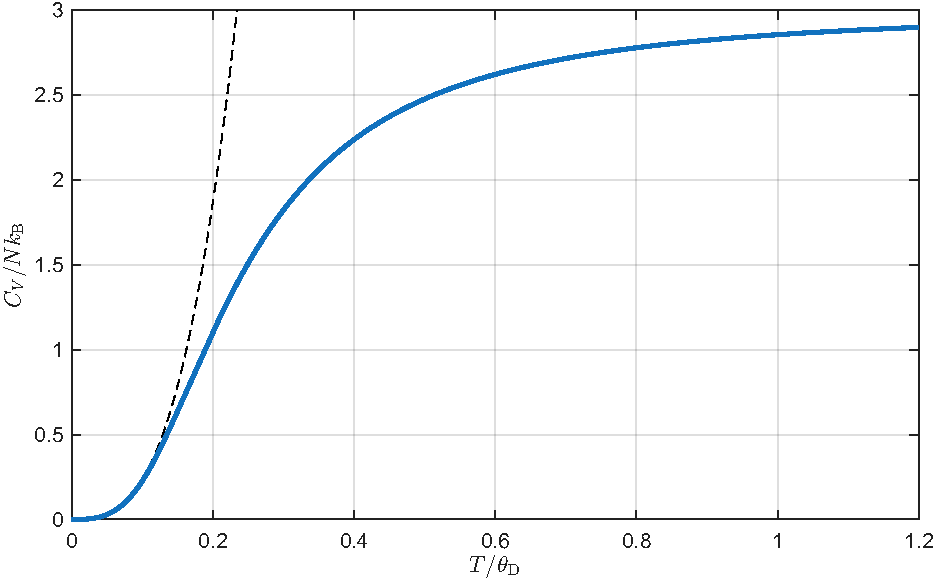
\includegraphics[width=0.8\linewidth]{figures/C_Vphonon.pdf}
	\captionof{figure}{声子气体热容$C_V$随温度的变化}
	\label{fig:CV phonon}
\end{notecaptionblock}

\begin{remark}
	~
\begin{compactenum}
	\item 固体中原子作用强，不能直接用近独立粒子统计。$T$较低时，简谐近似成立——原子集体振动的简正模式。
	相互独立：近独立的理想声子气体。
	\item 晶格中波矢为$\bm k$的声子具有能量$\hbar\omega$和晶格准动量$\hbar\bm k$。
	%但不同于电子等，
	在弱相互作用Bose气体中，长波密度振动的量子也称为声子。其色散关系由介质决定。
	\item 声学支在长波极限的频率趋于零。若一个原胞含多个原子，还可有原胞内原子相对振动的光学支。对色散较弱的光学支，可用Einstein模型近似其热容。金属的热容还含有导电电子的贡献。
\end{compactenum}
\end{remark}

\section{Fermi气体与Fermi液体}

\subsection{理想Fermi气体}

讨论简并费米气体的低温性质，
% $n\lambda_T^3\geqslant 1$，相互作用弱。
单个能级$\varepsilon_i$的量子态上的平均粒子数为
\[
	f_i:=\frac{a_i}{\omega_i}=\frac1{\e^{\alpha+\beta\varepsilon_i}+1}=\frac1{\e^{\beta(\varepsilon_i-\mu)}+1}.
\]

\paragraph{完全Fermi气}

% 讨论$T\to0$时电子的分布，
定义$T=0$时的化学势$\mu(0)=:\varepsilon_\Fermi$称为Fermi能量，则
\[
	\lim_{T\to0}f_i=\lim_{T\to0}\frac1{\e^{(\varepsilon_i-\mu)/\kB T}+1}=
	\begin{cases}
		1,&\varepsilon_i<\varepsilon_\Fermi\\
		0,&\varepsilon_i>\varepsilon_\Fermi
	\end{cases}
\]
由Pauli原理，粒子不能都处于$\varepsilon=0$态，但尽可能低，当$\varepsilon<\varepsilon_\Fermi$时，各量子态各有一个粒子；而$\varepsilon>\varepsilon_\Fermi$时，态无粒子。
Fermi能量可根据粒子数确定：
\begin{equation}
	N=\int_0^{\varepsilon_\Fermi}g(\varepsilon)\d\varepsilon=g_s\frac{2\pi V}{h^3}(2m)^{3/2}\cdot\frac23\varepsilon_\Fermi^{3/2}
	\implies
	\varepsilon_\Fermi=\frac{h^2}{2m}\biggp{\frac{3n}{4\pi g_s}}^{2/3}.
\end{equation}
进而可得
$T=0$时的零点内能、压强和熵
\begin{subequations}
	\begin{align}
		U_0&=\int_0^{\varepsilon_\Fermi}g(\varepsilon)\varepsilon\d\varepsilon=\frac35N\varepsilon_\Fermi,\\
		p_0&=-\pv{U_0}V=\frac23\frac{U_0}V=\frac25n\varepsilon_\Fermi,\\
		\lim_{T\to0}\frac SN&=0.
	\end{align}
\end{subequations}
在有限体系中，若最高占据能级恰好填满，则基态唯一且$S_0=0$。若这一简并能级只填入部分粒子，则有多种等能排布。三维均匀自由气体中，这类费米面上的简并对熵密度的贡献在热力学极限消失。

\begin{example}{金属中的电子气}{Electron Gas in Metals}
	电子$m_\electron\sim\qty{e-30}{\kilogram}$，数密度$n\sim\qty{e28}{\per\metre\cubed}$， % \tothe{3}
	自旋$g_s=2$，故$\varepsilon_\Fermi\sim\qty{1}{\electronvolt}$，
	\[
		v_\Fermi\sim\sqrt{\frac{2\varepsilon_\Fermi}m}\sim\qty[per-mode=symbol]{e6}{\metre\per\second}
	\]
	压强$p_0\sim\qty{e4}{\atm}$，这是纯粹的量子效应。
\end{example}

\paragraph{强简并Fermi气}

Fermi温度
\[
	T_\Fermi:=\frac{\varepsilon_\Fermi}\kB.
\]
对于金属电子气，$T_\Fermi\sim\qty{e4}{\kelvin}$。
低温情形$T\ll T_\Fermi$，热运动能量小，粒子分布基本不变，只有$\varepsilon_\Fermi\pm\kB T$附近的粒子可能是跳到高能级态上，如\figref{fig:strongly degenerate Fermi gas} 所示。
\begin{notecaptionblock}
	\tikzfigure{fermi-occupation}
	\captionof{figure}{强简并Fermi气粒子分布}
	\label{fig:strongly degenerate Fermi gas}
\end{notecaptionblock}
Fermi面附近能量宽度约为$\kB T$的区域内，有量级为$N T/T_\Fermi$的粒子可以被激发。每个激发所需的能量约为$\kB T$，因此
\[
	U-U_0\sim N\frac{T}{T_\Fermi}\kB T,\qquad
	C_V\sim N\kB\frac{T}{T_\Fermi}.
\]
要确定线性热容的系数，需同时满足粒子数约束。对$\mu$附近光滑的函数$\varphi(\varepsilon)$，在$\kB T\ll\mu$时作Sommerfeld展开：
\[
	\intRplus\frac{\varphi(\varepsilon)\d\varepsilon}{\e^{\beta(\varepsilon-\mu)}+1}
	=\int_0^\mu\varphi(\varepsilon)\d\varepsilon
	+\frac{\pi^2}{6}(\kB T)^2\varphi'(\mu)+\bigo(T^4).
\]
在固定$N,V$时，令$\delta\mu=\mu(T)-\varepsilon_\Fermi$。取$\varphi=g$并减去零温的粒子数积分，可得
\[
	0=g(\varepsilon_\Fermi)\delta\mu
	+\frac{\pi^2}{6}(\kB T)^2g'(\varepsilon_\Fermi)+\bigo(T^4).
\]
三维非相对论气体的$g(\varepsilon)\propto\sqrt{\varepsilon}$随能量增大，因此维持相同粒子数需要化学势略微下降。记$t=T/T_\Fermi$，有
\[
	\frac{\mu(T)}{\varepsilon_\Fermi}=1-\frac{\pi^2}{12}t^2+\bigo(t^4).
\]
再取$\varphi(\varepsilon)=\varepsilon g(\varepsilon)$计算内能，将积分上限的移动计入：
\begin{align*}
	U-U_0
	&=\varepsilon_\Fermi g(\varepsilon_\Fermi)\delta\mu
	+\frac{\pi^2}{6}(\kB T)^2
	\bigb{g(\varepsilon_\Fermi)+\varepsilon_\Fermi g'(\varepsilon_\Fermi)}+\bigo(T^4)\\
	&=\frac{\pi^2}{6}(\kB T)^2g(\varepsilon_\Fermi)+\bigo(T^4).
\end{align*}
由$g(\varepsilon_\Fermi)=3N/(2\varepsilon_\Fermi)$，得到
\begin{subequations}
	\begin{align}
		\frac{U-U_0}{N\varepsilon_\Fermi}&=\frac{\pi^2}4t^2+\bigo(t^4),\\
		\label{eqn:CV Fermi}
		\frac{C_V}{N\kB}&=\frac{\pi^2}2t+\bigo(t^3).
	\end{align}
\end{subequations}
\begin{notecaptionblock}
	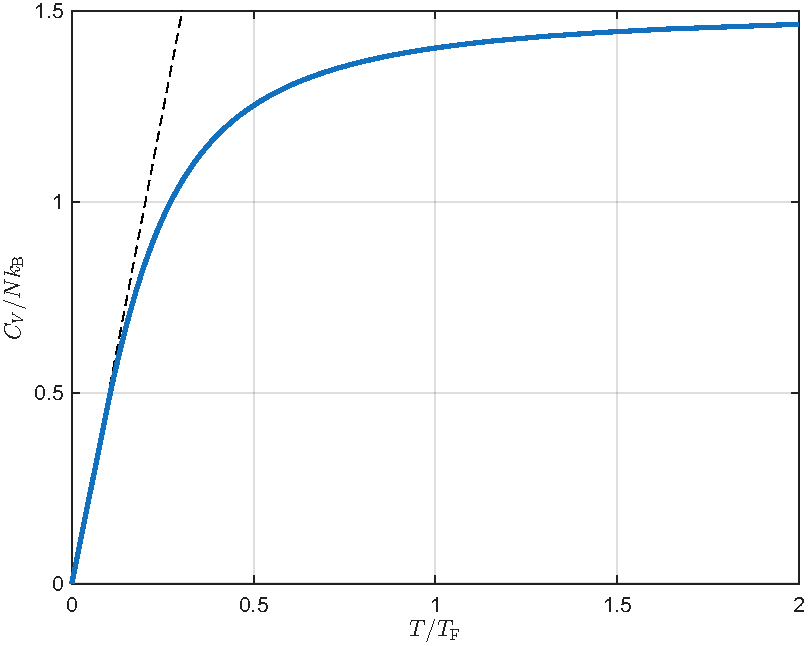
\includegraphics[width=0.8\linewidth]{figures/C_VFermion.pdf}
	\captionof{figure}{Fermi气体比热$C_V$随温度的变化}
\end{notecaptionblock}
因此低温下金属比热的实验值是电子气(Fermi气体)和晶格振动(Debye模型)共同贡献
\[
	C_V\simeq\underset{\text{Fermi}}{c_\electron T}+\underset{\text{Debye}}{c_\vib T^3}.
\]
与实验符合得很好。
\begin{example}{电子比热与晶格比热的比较}{}
	以每个原子贡献一个导电电子的金属为例，用$N$表示原子数。低温下，式\eqref{eqn:CV Debye}和式\eqref{eqn:CV Fermi}分别给出晶格与电子热容
	\[
	C_{V,\vib}=N\kB\frac{12\pi^4}5\Bigp{\frac T{\theta_\Debyelabel}}^3,\quad C_{V,\electron}=N\kB\frac{\pi^2}2\frac T{T_\Fermi}.
	\]
	对铜，$\theta_\Debyelabel\sim\qty{300}{\kelvin},\;T_\Fermi\sim\qty{8e4}{\kelvin}$，二者比值
	\[
		\frac{C_{V,\electron}}{C_{V,\vib}}=\frac5{24\pi^2}\frac T{T_\Fermi}\Bigp{\frac{\theta_\Debyelabel}T}^3\sim 7\Bigp{\frac{\qty{1}{\kelvin}}T}^2.
	\]
\end{example}

\subsection{Landau费米液体}
\label{sec:landau-fermi-liquid}

在液态$^3\mathrm{He}$中，原子间相互作用很强，低温正常相的热容却仍含有与$T$成正比的主项。Landau提出，如果逐渐接通相互作用时体系保持正常费米液相，低能的粒子或空穴激发可以与理想Fermi海中的激发一一对应。一个原子的运动会带动周围原子的重新分布，两者构成具有确定动量、能量及较长寿命的\textbf{准粒子}。这使Sommerfeld展开仍能用于低能热激发。\footnote{关于准粒子谱峰与Landau参数，见P.~A.~Lee的\href{https://ocw.mit.edu/courses/8-512-theory-of-solids-ii-spring-2009/resources/mit8_512s09_lec23_24/}{MIT 8.512固体理论讲义，第23、24讲}。}

\paragraph{费米面附近的寿命}
先取$T=0$，在费米面上方注入能量比化学势高$\xi$的准粒子。它与海中一个粒子散射后，末态含有费米面上方的两个粒子激发和费米面下方的一个空穴。由Pauli原理，这三个激发的能量代价均为正，且总和为$\xi$。把其中两个代价记为$x,y$，能量守恒固定第三个，则可用能量相空间正比于
\[
	\int_0^\xi \d x\int_0^{\xi-x}\d y=\frac{\xi^2}{2}.
\]
在三维正常费米液体中，若散射振幅光滑，角度积分给出有限系数。于是零温线宽$\Gamma=\hbar/\tau$正比于$\xi^2$，对空穴也有同一幂律。低温下费米面被展宽，在费米面上$\Gamma$正比于$(\kB T)^2$。沿$T=0$趋近费米面时$\Gamma/\abs{\xi}\to0$，因此准粒子能量越低，能量谱中的峰相对越窄。

\paragraph{热容测量有效质量}
对三维、各向同性的自旋$1/2$正常液体，费米面的体积由粒子数密度固定，故$p_\Fermi=\hbar(3\pi^2 n)^{1/3}$。在费米面附近把准粒子能量写成
\[
	\varepsilon_p^*-\mu\simeq v_\Fermi^*(p-p_\Fermi),\qquad
	m^*:=\frac{p_\Fermi}{v_\Fermi^*}.
\]
单位体积、单位能量的准粒子态数记为$\nu^*(0)$，其中零点取在化学势，两个自旋分量均已计入。对厚度为$\d p$的动量球壳计数可得
\[
	\nu^*(0)=\frac{2\cdot4\pi p_\Fermi^2}{(2\pi\hbar)^3v_\Fermi^*}
	=\frac{m^*p_\Fermi}{\pi^2\hbar^3}.
\]
费米面附近热激发的态密度在能量宽度$\kB T$内近似为常数。将前面的Sommerfeld展开应用于这些准粒子态，得到
\begin{equation}
	\frac{C_V}{V}=\gamma T+o(T),\qquad
	\gamma=\frac{\pi^2}{3}\kB^2\nu^*(0).
\end{equation}
在相同数密度下$p_\Fermi$相同，因此$\gamma$与质量为$m$的理想气体结果$\gamma_0$之比就是$m^*/m$。

\paragraph{核自旋磁化率测量准粒子相互作用}
$^3\mathrm{He}$原子的核自旋为$1/2$。记原子磁矩沿外磁场的两个投影为$\pm\mu_3$，其中$\mu_3>0$。令$s=n_+-n_-$为两种投影的数密度差，则磁化强度$M=\mu_3 s$。在固定总数密度下，两自旋分量的粒子密度分别改变$\pm s/2$。每个分量的态密度为$\nu^*(0)/2$，填充和腾空两层薄壳共需单位体积能量$s^2/[2\nu^*(0)]$。均匀极化还改变准粒子间的相互作用能，以无量纲系数$F_0^{\mathrm a}$表示它相对于该能量的大小。低温弱场下的自由能密度变化为
\[
	\delta f=\frac{1+F_0^{\mathrm a}}{2\nu^*(0)}s^2-\mu_3 B s .
\]
下标$0$表示费米面上均匀的角分量，上标$\mathrm a$表示两自旋分量反向变化的通道。稳定的顺磁态需有$1+F_0^{\mathrm a}>0$。对$s$极小化便得到核自旋磁化率
\[
	\chi_B:=\left.\pv{M}{B}\right|_{B=0}
	=\frac{\mu_3^2\nu^*(0)}{1+F_0^{\mathrm a}},\qquad
	\frac{\chi_B}{\chi_{B,0}}=\frac{m^*/m}{1+F_0^{\mathrm a}} .
\]
这里$B$是外加磁感应强度，$\chi_{B,0}$对应同密度、同核磁矩的理想气体。采用国际单位制的外场$H=B/\mu_0$时，无量纲的体磁化率为$\mu_0\chi_B$。在$^3\mathrm{He}$配对形成超流之前的低温正常相，可由热容斜率确定$m^*$，再由核自旋磁化率确定$F_0^{\mathrm a}$。两种测量共同区分了准粒子色散斜率的改变与均匀极化所需的相互作用能。\footnote{热容测量见\href{https://doi.org/10.1103/PhysRevB.27.2747}{D.~S.~Greywall, Phys.\ Rev.\ B \textbf{27}, 2747 (1983)}。核自旋磁化率测量见\href{https://doi.org/10.1103/PhysRev.128.509}{A.~Low Thomson等，Phys.\ Rev.\ \textbf{128}, 509 (1962)}。}
